\chapter{Introduction}
\label{ch:1}
\section{Introduction}
\label{sec-Introduction}
The following thesis investigates \acrlong{cl} as a framework for robust and efficient \acrlong{gw} analysis. \acrshort{cl} algorithms excel at incrementally learning from new data streams while retaining knowledge of previously encountered classes \citep{van2022three, qu2021recent, de2021continual}.\\
\acrshort{gw} are ripples in space-time caused by violent disruptions in the universe. Massive accelerating objects like \acrlong{ns} (\acrshort{ns}) and \acrlong{bbh} (\acrshort{bbh}) cause such strong waves propagating in all directions. Other cataclysmic events, responsible for \acrshort{gw}, are supernovae and obviously residues of the Big Bang \citep{CaltechWhatAreGW}. \\
Although the generation of \acrshort{gw} is a frenzy of energy, by the time the waves (invisible for the human eye) reach earth they are imperceptibly small.\\
The birth of \acrshort{ligo} (\acrlong{ligo}) offered a way to make very small measurements, equivalent to fractional changes in distance of $10^{-21}$ (smaller than an atom), microscopic measurements needed to detect \acrshort{gw} \citep{zevin2017gravity,glanzer2023data}. \\
\acrshort{ligo} has already completed three observing runs, abbreviated \acrshort{o1} (\acrlong{o1}), \acrshort{o2} (\acrlong{o2}) and \acrshort{o3} (\acrlong{o3}). At this very moment of writing the fourth observing run started on May the 24th of 2023 and the first period, 04a has ended on January the 16th of 2024 \citep{LIGORunPlan}. \\
Up to this point the types of uncovered \acrshort{gw} signals are limited to \acrshort{bbh}, \acrlong{bns} (\acrshort{bns}) and \acrlong{nsbh} (\acrshort{nsbh}) incidents. Researchers hope to unravel previously unseen cosmological cataclysms such as \acrshort{ccsne} (\acrlong{ccsne}), magnetars or probabilistic background waves from the Big Bang \citep{cuoco2020enhancing}. \\
\acrshort{gw} Analysis is a challenging field where scientists with varying backgrounds work together. With each observing run of \acrshort{ligo} resulting in more detected gravitational events (the majority were \acrshort{bbh} mergers) \citep{zevin2017gravity,glanzer2023data}, \citep{CaltechFAQ}. 

The accurate identification of \acrshort{gw} signals amidst noisy data remains a significant challenge. One of the primary sources of noise in \acrshort{gw} detectors are glitches. 
Glitches are short-lived non-Gaussian noise features that can be instrumental or environmental in nature. Glitches impact the analysis of wave candidates in three ways. Firstly, glitches increase the background loudness and thus reduce the candidate significance. Secondly glitches increase the uncertainty in the categorisation process because they operate with the same amplitude of astrophysical signals. Thirdly, the amount of usable data is even decreased more due to glitch contamination \citep{zevin2017gravity, cuoco2020enhancing}. \\
\acrlong{dl} (\acrshort{dl}) and especially \acrlong{cnn} (\acrshort{cnn}) have proven to be suitable architectures for extracting glitch features \citep{george2017deep,glanzer2023data,fernandes2023convolutional}. Together with the GravitySpy citizen science project \citep{bahaadini2018machine, zevin2017gravity}, the images can then be classified into their corresponding glitch morphologies, as seen in Figure \ref{fig:glitch_morphologies}.

\acrshort{gw} detectors host hundreds of thousands of auxiliary channels that monitor the state of the instruments and the environment. They have shown promise in characterizing glitches, such as \acrlong{idq} (\acrshort{idq}) \citep{essick2020idq,davis2022detector} or Elastic-net based ML for Understanding (EMU) \citep{colgan2020efficient} have been studied. The fusion of \acrfull{fd} analysis and \acrshort{ml} offers a robust framework for glitch detection in \acrshort{gw} analysis. Moreover, the scalability of \acrshort{fd} analysis across auxiliary channels holds promise for real-time glitch detection \citep{colgan2020efficient, benedetto2023ai}.

The limitations of the current classical approaches of offline training a neural network are evident due to the new data expected to be delivered in the fourth observing run \citep{wu2024advancing}. In this context, the field of \acrfull{il} or \acrshort{cl} emerges as a compelling area. The \acrshort{il} approach offers a fresh framework that allows models to learn from a continuously expanding dataset while still maintaining performance on previously encountered data \citep{van2022three, qu2021recent, de2021continual}.
Unlike batch learning, where models are trained on static datasets, \acrshort{cl} enables models to adapt incrementally to new data while retaining knowledge of previously encountered classes \citep{kirkpatrick2017overcoming}. 

In the context of \acrshort{gw} analysis, \acrshort{cl} strategies allow us to accommodate new glitch classes (as \acrshort{ligo} continues to operate and collect data, new glitch classes may emerge where \acrshort{cl} ensures that the model can seamlessly incorporate these novel classes without compromising performance on existing ones). It mitigates catastrophic forgetting (traditional \acrshort{ml} models tend to forget previously learned information when exposed to new data. \acrshort{cl} methods such as \acrfull{ewc} or memory-augmented architectures address this issue by preserving knowledge of existing glitch morphologies \citep{abbott2023open, kirkpatrick2017overcoming}.  

\begin{figure}[H]
    \centering
    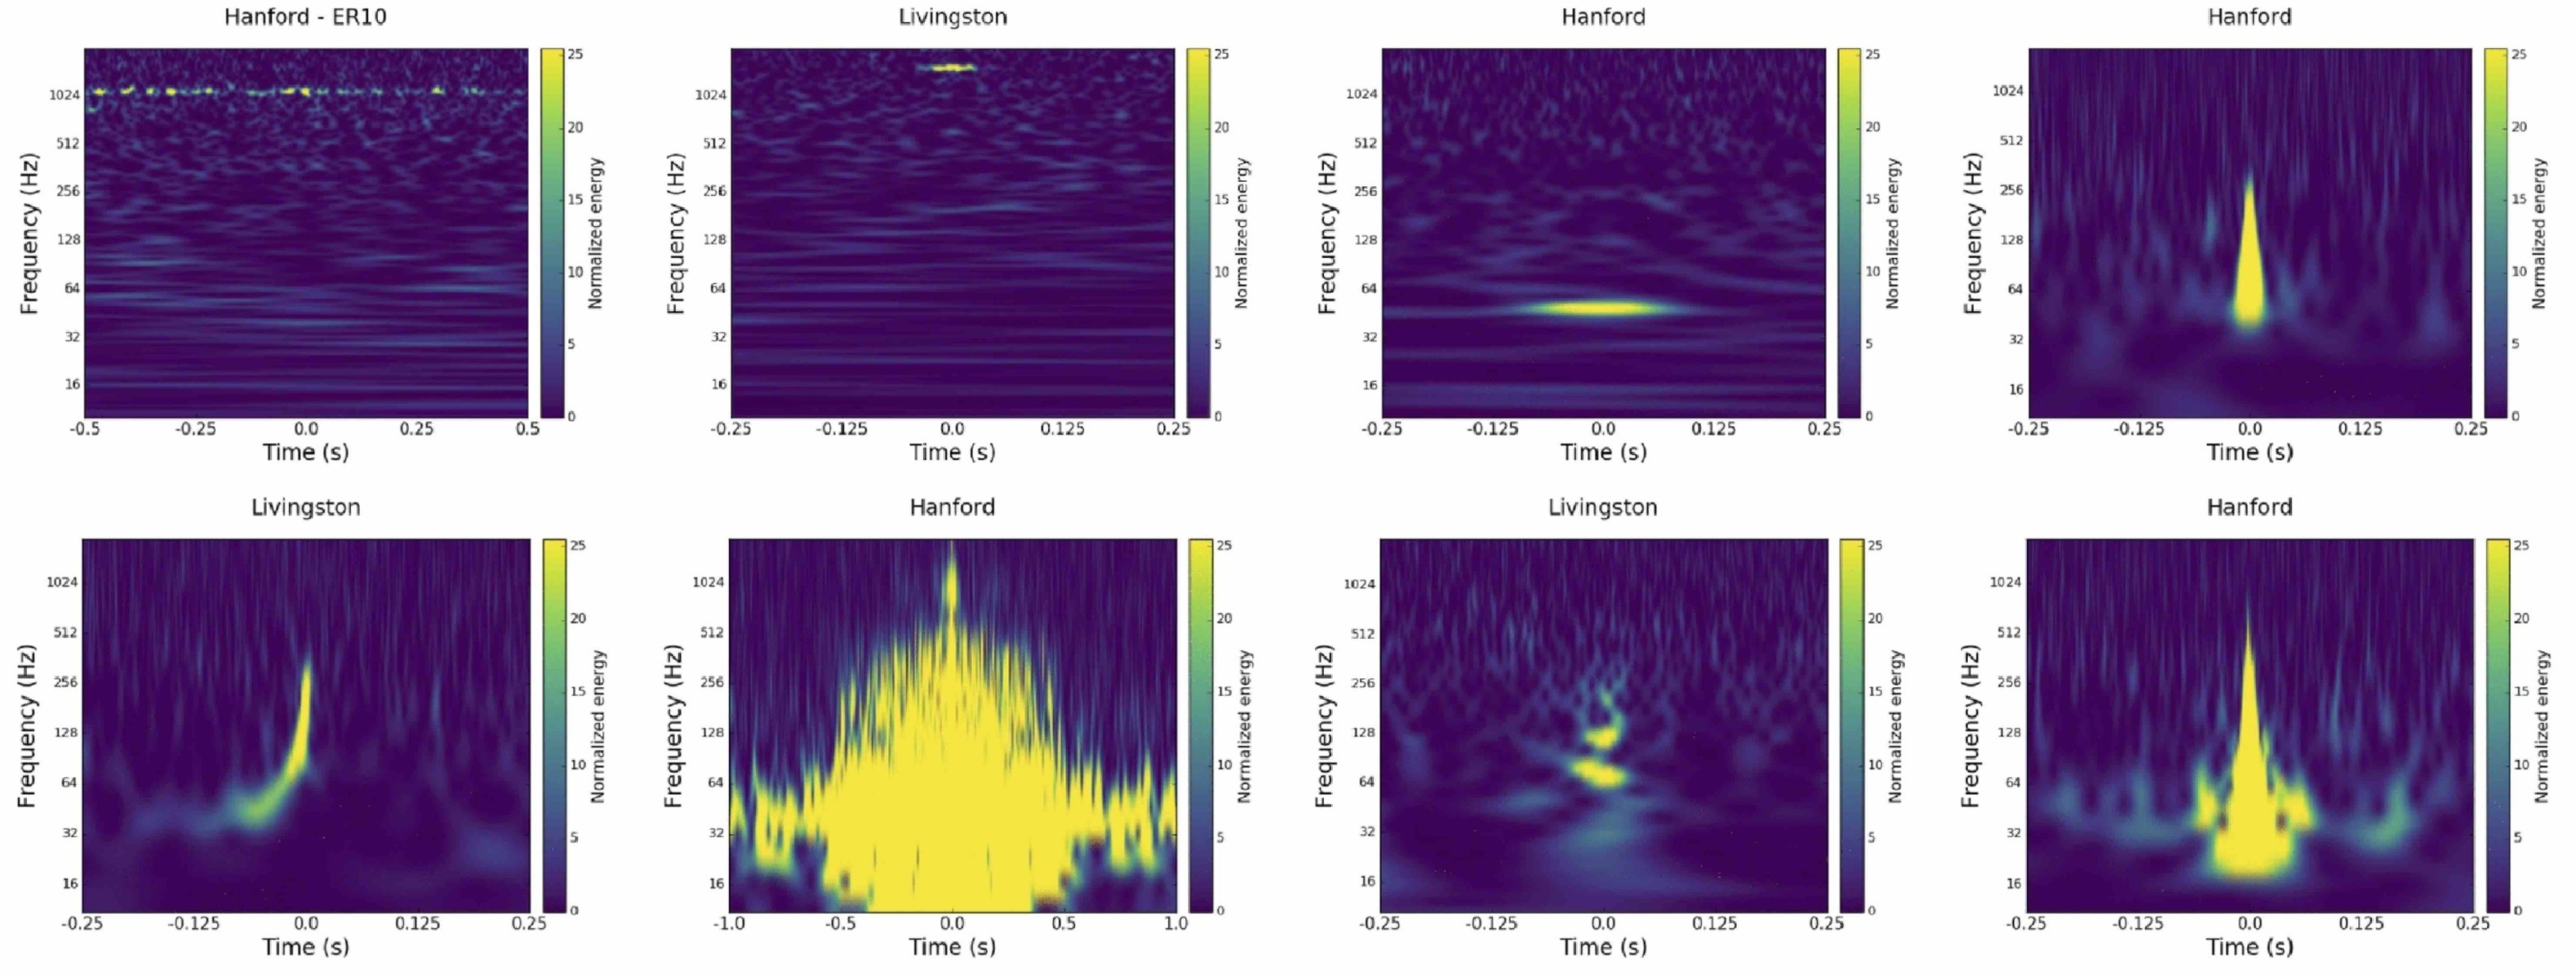
\includegraphics[width=0.8\textwidth]{Images/glitch_morphologies.jpg}
    \caption{Some glitch class morphologies. From top left to bottom right: 1080Lines, 1400Ripples, Air Compressor, Blip, row two: Chirp, Extremely Loud, Helix, Koi Fish. from \citep{glanzer2023data}}
    \label{fig:glitch_morphologies}
\end{figure}

In addition to identification and characterization of glitches, noise subtraction is another problem relating to signal processing \citep{benedetto2023ai, ormiston2020noise, davis2022detector, cornish2021bayeswave}. BayesWave is a tool that can be used to split the \acrshort{gw} signal from the noise \citep{cornish2021bayeswave}.

Glitches are only one side of the spectrum, it is evenly important that \acrlong{cbc} (\acrshort{cbc}) parameters can be correctly estimated. Researchers typically use waveform templates to compute the necessary parameter posteriors based on numerical solutions to the two body problem, but this remains computationally inefficient \citep{ajith2011addressing,coogan2022efficient,isoyama2020post}.

Searching GW signals is commonly split up in four separate categories. The first one being the \acrshort{cbc}'s (\acrshort{bbh}, \acrshort{bns}, \acrshort{nsbh}), the second type are called \acrshort{gw} bursts these can be the product of \acrshort{ccsne} or pulsar glitches. The third type are called long continuous \acrshort{gw}. The last category are residue waves from distant \acrshort{cbc}'s or even the Big Bang
\citep{abbott2020guide, LIGO_continuous}. The use of \acrlong{ml} (\acrshort{ml}), especially Random Forests (RF) was able to increase the detection speed of \acrshort{cbc}'s \citep{kapadia2017classifier}. The \acrlong{dl} (\acrshort{dl}) approach on the other hand has had mixed results \citep{gebhard2019convolutional,chatterjee2021extraction,ruan2023rapid}. 
Searching for other types of signals via \acrshort{ml} or \acrshort{dl} remains difficult because there is much uncertainty about morphology (due to lack of training data) \citep{cuoco2020enhancing}. 

A last application area where \acrshort{dl} is being investigated is the estimation of astrophysical parameters. Here Bayesian approaches have the ability to proof usefull, but the computational cost of calculating all posterior probabilities is an obstacle \citep{cuoco2020enhancing}.

\section{Thesis structure}
The thesis is structured as follows: 
\begin{enumerate}
    \item Introduction
    \item Related Work and Background
    \item Research Methodology
    \item Models and Results
    \item Discussion
    \item Conclusions and Recommendations
    \item Appendices
\end{enumerate}
\newpage



